\documentclass{beamer}

% Theme choice (you can change to Madrid, CambridgeUS, etc.)
\usetheme{Madrid}

% Optional packages
\usepackage[utf8]{inputenc}
\usepackage{graphicx} % for including images
\usepackage{amsmath, amssymb, mathtools} % for math symbols
\usepackage{hyperref} % for clickable links
\usepackage{tikz}

% Title info
\title[\texttt{/trading-presentation}]{Systematic Trading from First Principles}
\author[\texttt{github.com/odenpetersen}]{Oden Petersen}
\date{2025-10-31}

% Section headers
\newcommand{\sectionquote}[1]{\def\insertsquote{#1}}
\newcommand{\insertsquote}{}

\AtBeginSection[]{
	\begin{frame}
	\vfill
	\centering
	\begin{beamercolorbox}[sep=8pt,center,shadow=True,rounded=True]{title}
		\usebeamerfont{title}\insertsectionhead\par%
	\end{beamercolorbox}
	\vspace{1cm}
	{\Large\textit{\insertsquote}}\par
	\vfill
	\end{frame}

	\renewcommand{\insertsquote}{}
}

\begin{document}

% Title page
\begin{frame}
	\titlepage
	\begin{center}
		\textit{``$y=X\beta+\epsilon$, the rest is commentary.''}
	\end{center}
\end{frame}

\begin{frame}{About Me}
	\begin{itemize}
		\item UNSW Maths/Compsci (graduated T1 2025)
		\item Data Engineering @ Arnott's Biscuits (2021)
		\item CPMSoc Maths Director 2021
		\item Data Scientist @ Daisee (2021-2022)
		\item Started QuantSoc 2022
		\item Quant Intern @ Autumn Compass (2022)
		\item Quant Intern @ Citadel Securities (Summer 2023)
		\item Trading Intern @ Vivcourt Trading (Summer 2024)
		\item Starting work next year
		\item Polymarket trading go brr
	\end{itemize}
\end{frame}

\begin{frame}{Point of This Talk}
	\begin{itemize}
		\item Mathematise some intuitions about markets, trading systems, financial economics
		\item Give a precise picture of the many moving parts
		\item Build concepts axiomatically from the ground up
		\item Present a common basis for high-frequency and low-frequency trading (increasingly convergent)
		\item Starting point for exploring more resources. Like markets, a lot of financial literature is low-signal. \textit{``People without dirty hands are wrong.''}
	\end{itemize}

	Three approaches: systematic, semi-systematic, discretionary. Why systematic?
	\begin{itemize}
		\item Low-touch
		\item Consistency over time and across assets
		\item Low-latency opportunities
	\end{itemize}
	\textit{``We’re mediocre traders, but our system never has rows with its girlfriends.'' Nick Patterson, Renaissance Technologies}
\end{frame}

\begin{frame}{Not the Point of This Talk}
	\begin{itemize}
		\item How to get a job. In an efficient market the way to get a job is just to get good at the work
		\item How to do the job. The work itself is often extremely heuristic by necessity. The ability to appreciate which parts of the problem are most important represent things in a simple way while capturing the important qualitative parts is a key skill in both manual and systematic trading
		\item What the job is like. Communication at work focuses much more on concrete facts, relies on greater implicit shared context
		\item What you need to know for the job. Many of the best traders don't think in mathematical language
		\item The `correct' model for anything. Not all uncertainty is quantifiable (Frank Knight, Nassim Taleb). ``All models are wrong'' (George Box).
		\item Politics of financialisation and market structure
	\end{itemize}

\end{frame}
% Table of contents
\begin{frame}{Outline}
	\tableofcontents
\end{frame}

\sectionquote{``Governing by the power of virtue can be compared to the pole star, which remains fixed in place while all the other stars orbit respectfully around it.'' Confucius}
\section{Securities Markets}

\begin{frame}{Spot Transactions}
	The point of trading is to obtain an asset by giving up money, or obtain money by giving up an asset.

	If I give you $q>0$ units of some asset $A$, and you give me $\$pq$, then:%I'm gonna use dollar signs here although often we trade in many currencies. It is typical to emphasise one currency which we call the numeraire and express things in terms of it.
	\begin{itemize}
		\item I have \textbf{sold} $q$ units of $A$ to you at $\$p$
		\item You have \textbf{bought} $q$ units of $A$ from me for $\$p$
	\end{itemize} %"for" and "at" indicate direction

	Buying and selling are collectively called `trading'.%One trade can have multiple counterparties, we will see this later

	Suppose I own some amount of $A$ and some amount of money. If we let $s$ be $+1$ for buying and $-1$ for selling, then the result of any trade is to add $qs$ to the amount of $A$ I own, and add $-\$qps$ to the amount of money I have. %s is called the sign of the trade
\end{frame}

\begin{frame}{Securities Markets and Exchanges}
	The \textbf{\textcolor{blue}{market}} is the collective activity of all traders. When we don't care who we trade with, we can just `trade with the market'.

	A \textbf{\textcolor{red}{securities} \textcolor{blue}{market}} for some asset $A$, open at a time $t$, is any \textcolor{red}{standardised} \textcolor{blue}{way for traders to reach agreements to buy or sell} $A$ at a specified \textbf{settlement time} $T\geq t$. %"securities" because of standardisation and regulation. Agreements are often treated as the same as trades, though there are some cases where the distinction matters

	\pause

	For example, $T=\ldots$
	\begin{itemize}
		\item $t$ (`spot', e.g. blockchain) %ASX tried to do blockchain, this was scrapped in 2022 after 7yrs
		\item $t+1, t+2, \ldots$ (`clearing', e.g. equities)
		\item Last Thursday of month (`futures')
	\end{itemize}

	\pause
	If you agree to give something to someone, you have an \textbf{obligation}. If someone agrees to give you something, you have a \textbf{right}.

	\begin{block}{Counterparty Risk}
		If I have an agreement with $P_1$ to buy $10$ units for $\$p_1$ at $T$, and an agreement with $P_2$ to sell $10$ units at $\$p_2$ at $T$, and no further rights/obligations, am I guaranteed to meet my obligations?
	\end{block}%Define counterparty risk
\end{frame}

\begin{frame}{Centralisation}
	A \textbf{securities exchange} is a centralised venue serving a securities market for \textbf{exchange participants} (e.g. ASX, NYSE, TSE, HKEX, LME).

	Agreements not made through an exchange are often called OTC (over-the-counter). %Also called off-exchange. Define search costs.

	\begin{center}
		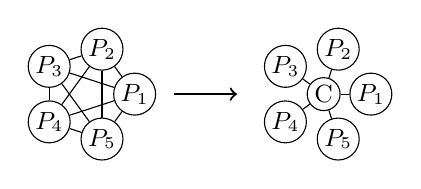
\begin{tikzpicture}[baseline, every node/.style={circle, draw, fill=white, inner sep=1pt, font=\small, minimum size=1mm}]
			\foreach \i in {1,...,5} {
				\node (n\i) at ({72*(\i-1)}:0.6) {$P_{\i}$};
			}
			\foreach \i in {1,...,5} {
				\foreach \j in {1,...,5} {
					\ifnum\i<\j
						\draw (n\i) -- (n\j);
					\fi
				}
			}

			\draw[->, thick] (1.1,0) -- (1.9,0);

			\begin{scope}[xshift=3cm]
				\node (c) at (0,0) {C};
				\foreach \i in {1,...,5} {
					\node (n\i) at ({72*(\i-1)}:0.6) {$P_{\i}$};
					\draw (c) -- (n\i);
				}
			\end{scope}
		\end{tikzpicture}
	\end{center}

	Centralisation generally reduces \textbf{search costs} and \textbf{counterparty risk}. %Mention risk counterexample: FTX vs a DEX
\end{frame}

\begin{frame}{Netting}
	Centralisation allows for \textbf{netting} of rights and obligations.

	For any settlement time $T$, I only need to keep track of the difference between money owed to and by me, and units owed to and by me.

	The quantity of $A$ owned by me, plus the quantity owed to me, minus the quantity owed by me to others, is known as my \textbf{net position} in $A$.

	If this is positive, I have a \textbf{long position}. If it is negative, I have a \textbf{short position}. If it is zero, I am \textbf{flat}.
\end{frame}

\begin{frame}{Collateralisation}
	At certain intermediate times $t'$ ($t\leq t'\leq T$), participants may be required to physically give (`post') something to the exchange to \textbf{collateralise} their obligations.
	\begin{itemize}
		\item Money (`margin') %Explain the term "futures type settlement" and "stock type settlement"
		\item Assets (`locate'/`borrow') %"Borrow" is only if you don't own the thing
	\end{itemize}
	If an agreement made on the exchange gives you rights to money or assets at $T$, this is typically as good as posting actual money or assets for an obligation at $T'\geq T$.

	Some amount of interest may be charged to make up for the difference between the size of our obligations and the size of our collateral. For cash, this is according to an \textbf{interest rate}; for other assets, it is according to a \textbf{borrow rate}/\textbf{short rate}.
\end{frame}

\begin{frame}{Summary}
	\begin{itemize}
		\item \textbf{Trading} is swapping money and assets
		\item A \textbf{market} is whatever you use to trade
		\item A \textbf{securities market} is a standardised way to agree to trades
		\item Agreements consist of \textbf{rights} and \textbf{obligations}
		\item Finding a \textbf{counterparty} may involve \textbf{search cost}
		\item Agreements between two parties are subject to \textbf{counterparty risk}
		\item A \textbf{securities exchange} is a centralised trading venue %Maybe explain national market system
		\item After trades are agreed to on an exchange, they will be \textbf{settled} in some standardised way
		\item The net quantity of $A$ that I have some claim to can either be positive (\textbf{long position}), negative (\textbf{short position}), or zero (\textbf{flat}).
		\item Traders may be obligated to post assets ('locate') or money ('margin')
	\end{itemize}
\end{frame}

\sectionquote{``To gain an advantage from better knowledge of facilities of communication or transport is sometimes regarded as almost dishonest, although it is quite as important that society make use of the best opportunities in this respect as in using the latest scientific discoveries.'' Hayek}
\section{Trading}
\begin{frame}{Setup}
	A sequence of trades that collectively increases the amount of money you have and leaves the amount of each asset you have unchanged is clearly favourable.

	\pause

	Suppose that at each time $t$ we have cash holdings of $\$c_t$ and net holdings of $a_t$ units of some asset $A$.

	Suppose also that trades $(s_t, q_t, \$p_t)$ take place at a finite set of distinct times
	$$\tau = \{t_1,\ldots t_n\}\subset T = [t_-, t_+],$$
	where $t_-<t_1<\ldots<t_n<t_+$.

	\pause

	Suppose further that $p_t$ is a right-continuous function $\mathbb R\to\mathbb R$ with left-limits.

	For instance, we could take $p_t = p_{\max \left(\tau\cap (-\infty,t]\right)}$ for $t\geq \min\tau$ and $p_t=x$ otherwise for some arbitrary $x$. This is known as the last traded price.
\end{frame}

\begin{frame}{Accounting}
	For any time-varying quantity $x_t$, let $x_t^+$ and $x_t^-$ denote the right- and left-limits respectively.

	Furthermore, define a signed measure $x_\omega$ such that for any interval $T'=[t_-',t_+']$ we have
	$$x_{T'} := x_{t_+}^+ - x_{t_-}^-.$$

	\pause

	Then we have

	\vspace{-0.06\textheight}
	\begin{align*}
		a_{T'}	&= \sum_{t\in \tau} s_t q_t		&&= \int_{t\in T} da,
	\\	c_{T'}	&= \sum_{t\in \tau} - p_t (s_t q_t)	&&= \int_{t\in T} - p_t da,
	\\	p_{T'}	&= p_{t_+'} - p_{t_-'}^-.		&&= \int_{t\in T} dp.
	\end{align*}%Special case: t_-'=t_+'
\end{frame}

\begin{frame}{Cash Holdings}
	It can be shown (see appendix) that the cashflow over the entire interval $T=[t_-,t_+]$ is
	$$\$c_T = \int_{t\in T} - \$p_t da = \$p_{t_-}a_{t_-} - \$p_{t_+}a_{t_+} + \$\int_{t\in T} a_t^- dp.$$
	This is similar in spirit to integration by parts:
	$$\int_a^b f \frac{dg}{dx} dx = f(b)g(b)-f(a)g(a) - \int_a^b g \frac{df}{dx} dx.$$

	Then we have
	$$\$(c_{t_+} + p_{t_+}a_{t_+}) - \$(c_{t_-} + p_{t_-}a_{t_-}) = \$\int_{t\in T} a_t^- dp.$$

	The quantity $\$v_t = \$p_t a_t$ is known as the \textbf{dollar value} of our $A$ holdings \textbf{marked} to the price $\$p_t$.%Marking just means multiplication of units held by a unit price
\end{frame}

\begin{frame}{Portfolio Valuation}
	Suppose now that we trade multiple assets, such that $p_t$, $a_t$ and $v_t$ are vector-valued, with $v_t$ the elementwise product of $p_t$ and $a_t$.

	A collection of assets held in quantities $a_t$ is known as a \textbf{portfolio}.

	We can write
	$$\$(c_{t_+} + p_{t_+} \cdot a_{t_+}) - \$(c_{t_-} + p_{t_-} \cdot a_{t_-}) = \$\int_{t\in T} a_t^- \cdot dp,$$
	where $p_\omega$ is now a vector-valued measure. \pause Let
	$$\$\Pi_t = \$c_t + \$p_t\cdot a_t = \$c_t + \$\sum v_t.$$

	We call $\$\Pi_t$ the \textbf{value} of our portfolio \textbf{marked} to $p_t$.
\end{frame}

\begin{frame}{Profitability}
	The quantity $\$\Pi_{t_+} - \$\Pi_{t_-}$ is our \textbf{net P\&L} (profit and loss) over the interval $T$, marked to $p_t$.
	Then we have
	$$\Pi_T	= \int_{t\in T} a_t^- \cdot dp.$$
	we can write
	$$\Pi_{[t_i,t_{i+1}]} = \int_{[t_i,t_{i+1}]} a_t^- \cdot dp = \int_{t\in [t_i, t_{i+1}]} v_t^- \cdot \frac{dp}{p_t^-},$$
	where the quotient $\frac{dp}{p_t^-}$ is computed elementwise.
\end{frame}

\begin{frame}{Leverage}
	Suppose we can always make any trade we like at time $t$ with price $\$p_t$ (in practice, there are limits on the trades we can make at a particular price and time). %Not a terrible guess if we did indeed make some trade at $\$p_{t_i}$.

	Then we can freely convert a portfolio with value $\$\Pi_t$ to that much in cash.

	Conversely, we can convert $\$\Pi_t$ worth of cash into any portfolio with that value.

	\pause

	Typically, $\$\Pi_t$ can change in two ways: trading assets, or transferring cash into and out of the portfolio. We will generally ignore the possibility of transfers.

	If we begin with a portfolio worth $\$\Pi_{t_1}$ and make a sequence of trades of the form $(s_t,q_t,p_t)$ that result in a portfolio worth $\$\Pi_{t_n}$, then we could instead begin with a portfolio worth $L \$\Pi_{t_1}$ and make trades $(s_t, L q_t, p_t)$ to arrive at a portfolio worth $L \$\Pi_{t_n}$. The ratio $L$ is known as the \textbf{leverage ratio}.
\end{frame}

\begin{frame}{Return on Capital}
	Because of collateralisation requirements, portfolio management uses up cash.

	Consider long-only spot-settled trading. If we were to turn our portfolio into cash, or convert cash into an identical portfolio, we would receive/require $\$\Pi_t$.\footnote{We generally want $c_t$ to be small, but we may want some spare cash for trading, so it still forms part of the collateralisation requirement.}%For a long-short portfolio with no borrow costs, the collateral requirement is generally at least $c_t + \vert a_t\vert \cdot c_t$. The calculations are different for margined trading eg futures. Complexity i wont go into. Maybe appendix?

	%To judge trading efficiency, we might want an estimate for how much extra P\&L over the interval $T$ would result from a marginal dollar added to $\$\Pi_t$.

	If our initial portfolio value were $\$\Pi_{t_-}+\$N$ instead of $\Pi_{t_-}$, and we could simply scale up trade sizes at the same prices, then set
	$$L = \frac{\Pi_{t_-}+N}{\Pi_{t_-}}.$$

	The \textbf{return on capital} is defined as the increase in P\&L per dollar added to initial portfolio value, i.e.
	$$R_T = \frac{L \int_T d\Pi - \int_T d\Pi}{N} = \frac{\int_T d\Pi}{\Pi_{t_-}}.$$
\end{frame}

\begin{frame}{Log Returns}
	If we define
	$$\ell_t = \log \Pi_t,$$ %sometimes called log-wealth
	then for any interval $T'=[t_-',t_+']$, we have
	$$\ell_{T'} = \log\left(\frac{\Pi_{t_+'}^+}{\Pi_{t_-'}^-}\right)= \log(R_{T'}+1),$$
	and so
	$$R_{T'} = \exp(\ell_{T'}) - 1.$$
	Then for any measurable set $\omega$ we can define
	$$R_\omega = \exp(\ell_\omega) - 1 \approx \ell_\omega + O(\ell_\omega^2)\textrm{ (for small }\ell_\omega\textrm{)}.$$

	We call $\ell_T$ the \textbf{log-return} over the interval $T$.
\end{frame}

\begin{frame}{Properties of Returns and Log-Returns}
	Let $w_t := \frac{1}{\Pi_t}v_t$ be the \textbf{weight vector}.%Explain interpretation

	For an interval $T' = (t_i,t_{i+1}]$, we have $a_t^-$ equal to a constant over $T'$, and
	$$R_{T'} = w_{t_i}^+ \cdot r_{T'},$$
	where the elementwise quotient
	$$r_{T'} = \frac{p_{t_{i+1}} - p_{t_i}}{p_{t_i}}$$
	is known as the \textbf{asset returns} vector over $T'$. In contrast, $\ell_{T'}$ is not linear in $r_{T'}$. %In fact there's no function of the return that \ell_{T'} is linear in. Benefits and drawbacks, eg expectation/variance

	For a disjoint collection of measurable sets $\omega_1,\ldots\omega_n$ whose union is $\Omega$, we have
	$$\ell_\Omega & &= \sum_{i=1}^n \ell_{\omega_i},$$
	$$R_\Omega &= \left(\prod_{i=1}^n (1+R_{\omega_i})\right) - 1 &\approx \sum_{i=1}^n R_{\omega_i} + O\left(\sum_{i=1}^n\sum_{j=1}^n \vert R_{\omega_i} R_{\omega_j} \vert\right).$$
\end{frame}

\begin{frame}{Summary}
	\begin{itemize}
		\item A sequence of trades that increases $c_t$ without changing $a_t$ is almost always a good thing
		\item Trades $(s_t,q_t,\$p_t)$ will take place at discrete times $\tau$
		\item P\&L marked to $p$ is $\$\Pi_T = \int_{t\in T}a_t^-dp$
		\item \textbf{Portfolio returns} are the percentage change in $\Pi_t$
		\item Portfolio returns are the dot product of \textbf{portfolio weights} and \textbf{asset returns}
		\item \textbf{Portfolio log-returns} are the change in $\log\Pi_t$
		\item Log-returns and returns are approximately equal when small
		\item Log-returns are additive over time
	\end{itemize}
\end{frame}

\sectionquote{``Certainly, the modern compendium of mental illnesses (DSM-5) takes a dim view of people who think everyone is out to get them. Yet financial markets are different: people really are out to get you, after all.'' - Agustin Lebron, The Laws of Trading}
\section{Market Microstructure}
\begin{frame}{Trade Formation}
	In practice, the trades we can make at a time $t$ and a price $p_t$ are limited by our ability to find a willing counterparty.

	On an electronic exchange, trades are formed by interacting with the exchange's \textbf{matching engine}.%Matching engine is a computer networked with the computers of exchange participants. Usually the algorithm is mostly deterministic and publicly known, but this is not always the case and knowledge of the matching engine can give you an advantage over other traders

	\pause

	For each trade $(s,q,\$p)$, the exchange will typically charge a fee proportional to the \textbf{dollar volume} $\$pq$ of the trade. Fee rates may vary depending on trade type and between participants in accordance with exchange policy.

	\pause

	The most common type of matching engine design is a \textbf{limit-order book} (sometimes called a double auction), which can operate in either a \textbf{continuous} or \textbf{batched} fashion.
\end{frame}

\begin{frame}{Limit Order Book}%Special kind of data structure
	At any point in time, market participants can create a request (`\textbf{limit order}') of the form $(s,q,\$p)$ to trade up to $q$ units in direction $s=\pm1$ at any price $\$(p-sm), m\geq0$.%If I'm happy to buy for at most 10 then I'm happy to buy for 1 since this would be a price improvement of 9

	The value $\$m$ is known as the \textbf{price improvement}. %The request poster prefers large m. $p is sometimes called the reserve price
	
	They are then said to be ``\textbf{bid} for $\$p$'' ($s=+1$) or ``\textbf{ask}ing/\textbf{offer}ing at $\$p$'' ($s=-1$). %Bid and ask are terms referring to limit order directionality. for and at also indicate direction, as mentioned before

	\pause

	All limit orders active at time $t$ are collected into a \textbf{limit-order book} $\mathcal{L}_t$. By convention, $\mathcal{L}_t$ is right-continuous with left limits.%multiset

	Users can add, cancel and modify orders, subject to exchange-specific rules.%Limits on modification. Ratelimits, message limits etc. GFD etc - FOK FAK explained later
\end{frame}

\begin{frame}{Order Matching}
	Whenever $(+1,q_1,\$p_1), (-1,q_2,\$p_2)\in\mathcal{L}_t$ with $p_2\leq p_1$, both orders could be at least partly satisfied by trading up to $q_{\max}=\min(q_1,q_2)$ units with one another at a price $\$p\in[\$p_2,\$p_1]$. If such a pair exists the book is said to be \textbf{in cross}.

	\pause

	If an order $(s,q,\$p)$ is in cross with another, it may be \textbf{matched} for $q'$ units. The total matched quantity for all buy orders must equal the total matched quantity for all sell orders.

	In this case, $q'$ units will trade, and the order will become $(s,q-q',\$p)$.

	If $q=q'$ the order is said to be \textbf{fully filled} and will be removed from the book. Otherwise, it is said to be \textbf{partially filled}.

	The ability to quickly find matches for a large number of units at a reasonable price is known as \textbf{liquidity}, and is another major benefit of centralisation.
\end{frame}

\begin{frame}{Supply and Demand Curves}
	We can partition $\mathcal{L}_t$ into $\mathcal{L}_t = \mathcal{B}_t\cup\mathcal{A}_t$, with $\mathcal{B}_t$ the bid orders and $\mathcal{A}_t$ the ask orders.

	\pause

	Now define the functions
	\begin{align*}
		Q_t(+1,\$p)	&= \sum_{\substack{(+1,q',\$p') \in \mathcal{B}_t \\ \$p\leq \$p'}} q'
	\\	Q_t(-1,\$p)	&= \sum_{\substack{(-1,q',\$p') \in \mathcal{A}_t \\ \$p\geq \$p'}} q'
	\\	M_t(\$p)	&= \min(Q_t(+1,\$p),Q_t(-1,\$p))
	\end{align*}
	\pause
	The functions $Q_t(-1,\$p)$ and $Q_t(+1,\$p)$ are known as the \textbf{supply curve} and \textbf{demand curve} respectively. The function $M_t(\$p)$ represents the \textbf{matchable quantity} at $\$p$.
	\pause
	The book $\mathcal{L}_t$ is in cross if and only if there exists some $\$p$ with $M_t(\$p)>0$.
	%Diagram. separate slide
\end{frame}

\begin{frame}{Batch Matching}
	In \textbf{batch} or \textbf{auction} style matching, orders are matched with one another only at particular discrete times.

	\begin{enumerate}
		\item Prior to the \textbf{match time} $t^*$, users can typically add, modify and cancel limit orders.
		\item At each time $t\leq t^*$, an \textbf{indicative price} $\$p^*_t$ will be selected such that $M_t(\$p^*_t)$ is maximal. Tiebreaking will depend on exchange rules.
		\item Finally, at the match time $t^*$, some subset of the crossed limit orders will be matched at $\$p^*$ for a total quantity $M_{t^*}(\$p^*_{t^*})$. After the match, the book will no longer be crossed.
	\end{enumerate}

	\pause

	Maximising $M_t(\$p^*_t)$ is equivalent to maximising the sum of $\$qm$ across all orders, where $q$ is the quantity filled and $m$ is the price improvement.%Also maximises fees paid

	It is common to use this matching style at the beginning or end of a trading day or lunch break, or when there is some kind of market instability such as following a large price move or company announcement. Sometimes $t^*$ is referred to as a \textbf{liquidity event} because of the large volume traded, and the relative insensitivity of $\$p^*_{t^*}$ to individual orders.%Price impact nonnegative because of monotonicity property
\end{frame}

\begin{frame}{Batch Matching Properties}
	The following monotonicity properties typically hold:
	\begin{itemize}
		\item $\$p^*_t$ nondecreasing in $\mathcal{B}_t$ and nonincreasing in $\mathcal{A}_t$
		\item For each $\$p$, $M_t(\$p)$ nondecreasing in $\mathcal{L}_t$
		\item For individual orders $(s,q,\$p)$, we will have $\$p^*_t$ nondecreasing in $\$p$ and $sq$. %The sensitivity of the match price to the parameters of the individual order is known as the instantaneous price impact.
		\item For individual orders $(s,q,\$p)$ and each $\$p'$, we will have $M_t(\$p')$ nondecreasing in $q$ and nondecreasing in $\$sp$.
	\end{itemize}

	\pause

	\begin{block}{Price Priority}
		Because $M_t(\$p')$ is nondecreasing in $sp$, the matching will be designed to obey \textbf{price priority}.
	
		If we have two orders $(s_1,q_1,\$p_1), (s_2,q_2,\$p_2)$ with $\$s_1p_1 > \$s_2p_2$, then the second order cannot be matched unless the first is completely filled.
	\end{block}
\end{frame}

\begin{frame}{Order Timing}
	The order book is often visible to all participants. Traders may be incentivised to wait until immediately before the match time to post orders.%Hiding intentions, using all information available

	If everyone does this, the matching engine may be overloaded, and $p^*_t$ will change very rapidly leading up to $t^*$.

	\pause

	The match time is typically chosen at random in some short interval in order to disincentivise this behaviour.
\end{frame}

\begin{frame}{Time Priority}
	To further encourage early submission of orders, many exchanges also implement a time priority rule.%As opposed to pro rata
	\begin{block}{Time Priority}
		If two orders exist at the same price $\$p$, the one that reached the matching engine later cannot be matched unless the earlier order is completely filled.
	\end{block}

	\pause

	\begin{block}{Tick Size}
		Time priority would not have much effect if we could just insert the later order at a price $\$p+s\epsilon$ for some very small $\epsilon>0$.%Because of price priority. "Diming"

		To avoid this, prices must be integer multiples of some small increment $\$\delta$, known as the \textbf{tick size}.%Sub-penny rule reg nms
	\end{block}
\end{frame}

\begin{frame}{Continuous Matching}
	In \textbf{continuous matching}, a match time is triggered every time a new limit order causes the book to become crossed.

	Price priority is still used, and time priority is usually used.

	This is mainly used for intraday trading, night session trading, and 24/7 markets like crypto.

	If the matching engine receives an order at $t$, then immediately before and after $t$ the book will be uncrossed, with $M_t(\$p)=0$ at all $\$p$.

	\pause

	The only orders involved in the match will be the arriving order and some set of orders $\mathcal{M}_t$ in the opposite direction.

	Typically we are not allowed to match with ourselves. Often the exchange will implement \textbf{self-trade protection} so that the quantity of our active and passive orders is simply cancelled out without recording a trade.
\end{frame}

\begin{frame}{Order Types}
	The arriving order is known as the \textbf{active} or \textbf{aggressive} order, and the pre-existing orders are known as \textbf{passive}.%Also known as taker and maker orders. Sometimes have different fees

	\pause

	Depending on the price, the active order may not be fully filled. The rest will be converted to a passive order. We can avoid this by specifying a \textbf{fill-or-kill} or \textbf{fill-and-kill} order type.

	\pause

	If we don't care about price, we can insert a market order $(s,q,s\infty)$. The traded price can be arbitrarily bad for us, so this is rarely a good idea.

	\pause

	Passive orders give all participants the option to trade at a particular price in the opposite direction.%Exchanges want to incentivise liquidity

	However, they disappear when traded against, so it is important to be fast if we think other traders will behave similarly to us.%Latency
\end{frame}

\begin{frame}{Latency}
	If we are too slow, we will only make a trade when faster participants have decided it is unfavourable. This is known as \textbf{adverse selection}.

	\pause

	If we are too slow to cancel our passive orders, they will be traded against even when we have already decided this is no longer favourable.

	\pause

	If we are slow to cancel, we will need to make the decision to cancel based on less information. This will increase the frequency with which we regret cancelling an order due to loss of queue priority.

	\pause

	We can respond more quickly to events on the exchange by paying for \textbf{colocation}, writing faster code, using specialised hardware (fibre optic, FPGAs), or exploiting aspects of exchange design.

	Latency can sometimes be nontrivial to quantify due to \textbf{clock drift}, which may need to be smoothed out.
\end{frame}

\begin{frame}{Trades Resulting from Continuous Matching}
	For each $q'$ matched against a passive order $(s,q,\$p)$, the active order will trade $q'$ units with the passive order at $\$p$. %Unlike auction-style matching, there may be multiple trade prices according to the prices of the passive orders. No price improvement for passive orders

	The per-unit price achieved by the active trader will be
	$$\$p^*_t = \frac{\sum_{(s,q,\$p)\in\mathcal{M}_t} \$pq}{\sum_{(s,q,\$p)\in\mathcal{M}_t} q}.$$ %This may or may not be a multiple of the tick size.
\end{frame}

\begin{frame}{Instantaneous Price Impact}
	If we aggressively trade a very large quantity, we will exhaust all passive orders we would most prefer to trade with and $\mathcal{M}_t$ will need to include orders at worse price levels. This is sometimes known as \textbf{walking the book}.

	Assume continuous matching, and consider a market order of $q>0$ units in direction $s$.

	The least favourable price in $\mathcal{M}_t$ will be given by
	$$\$P_t(sq) = s\min_{\{\$p : Q_t(-s,p)\geq q\}} \$sp.$$

	The unit price of the match will be given by
	$$\$p^*_t(sq) = \frac{1}{q}\int_0^q \$P_t(sq')dq'.$$

	We call the sensitivity of $\$p^*_t$ to $sq$ the \textbf{instantaneous price impact}.%Sometimes known as transient price impact
\end{frame}

\begin{frame}{Bid-Ask Spread}
	We call the prices
	\begin{align*}
		\$b_t	&= \lim_{q\to0^+} \$p^*_t(-q)	&&= \max_{(+1,q,\$p)\in\mathcal{B}_t} \$p
	\\	\$a_t	&= \lim_{q\to0^+} \$p^*_t(q)	&&= \min_{(-1,q,\$p)\in\mathcal{A}_t} \$p
	\end{align*}
	the \textbf{bid price} and \textbf{ask price} respectively. All bid orders have price at most $\$b_t$ and all ask orders have price at least $\$a_t$.%To trade an infinitesimal amount, we would need to sell at $\$b_t$ or buy at $\$a_t$.

	The interval $[\$b_t,\$a_t]$ is known as the \textbf{spread}, and $\$a_t-\$b_t$ is the \textbf{width} of the spread. If $\$a_t-\$b_t=\$\delta$, we say that the market for the asset is \textbf{large-tick} or \textbf{tick-constrained}.%Proxy for liquidity
\end{frame}

\begin{frame}{Arbitrage}
	Suppose the same asset (or extremely similar assets) can be traded in two separate order books $\mathcal{L}_t^1, \mathcal{L}_t^2$ with spreads $\delta_1 = [\$b_1,\$a_1]$ and $\delta_2 = [\$b_2, \$a_2]$.

	If $\delta_1\cap\delta_2=\emptyset$ (i.e. if $a_1<b_2$ or $a_2<b_1$), then $\mathcal{L}_t^1\cup\mathcal{L}_t^2$ is in cross. We can buy from one book and immediately sell to the other book for a higher price. This is known as \textbf{cross-listing arbitrage}.

	Our positions will probably not be netted by the exchange. So this may require collateral. If the order books get close together we may be able to get out of the position. If they get further apart we may require even more collateral, or need to exit the position at a loss.%ETF creation redemption

	We will also need to take into account fees. For a fee rate $f$ we can adjust the spreads to be $[(1-f)\$b_t,(1+f)\$a_t]$.

	If $\mathcal{L}_t^1$ or $\mathcal{L}_t^2$ changes before our order reaches the matching engine, we may not get the fill, or the price may no longer be favourable.

	Even if $\delta_1\cap\delta_2\not=\emptyset$, it may be possible to make one of the trades passively, and make the other immediately after the first is filled.%Also PFOF
\end{frame}

\begin{frame}{Price Proxies}
	Note that $\$p^*_t(0)$ is not yet defined. So long as we choose some price $\$m_t$ satisfying $\$m_t\in[\$b_t,\$a_t]$, setting $\$p^*_t(0) := \$m_t$ will make $\$p^*_t(\cdot)$ nondecreasing.

	This is variously called the \textbf{theo}retical price, \textbf{microprice} or \textbf{price proxy} depending on context.

	\pause

	It is well known that the last traded price $\$p_t$ exhibits \textbf{negative serial autocorrelation} of returns $\frac{dp}{p_t^_}$ (sometimes called \textbf{bid-ask bounce}).

	Most price proxies exhibit some degree of statistical predictability that cannot be exploited for profit. This is known as \textbf{microstructural noise}.

	%Diagram of Roll model
\end{frame}

\begin{frame}{Common Microprices}
	Some simple choices for $m_t$ include:
	\begin{itemize}
		\item $\frac{1}{2}b_t+\$\frac{1}{2}a_t$ (arithmetic \textbf{midprice})
		\item $\$\sqrt{b_ta_t}$ (\textbf{geometric midprice})
		\item $\$(1-I_t)b_t + \$I_ta_t$ (depth-$\$d$ \textbf{weighted midprice})
		\item $\$b_t^{1-I_t}a_t^{I_t}$ (depth-$\$d$ \textbf{geometrically weighted midprice})
	\end{itemize}
	We call $I_t$ the \textbf{book imbalance}.

	\pause

	A popular choice for this is
	$$I_t=\frac{Q_t(+1,\$b_t)}{Q_t(+1,\$b_t)+Q_t(-1,\$a_t)}.$$

	Alternative price proxies are described in the appendix.
\end{frame}

\begin{frame}{Persistent Price Impact}
	We call the difference $\$\lambda_t(sq) = \$p^*_t(sq) - \$m_t$ the \textbf{instantaneous price impact curve} of trading $q$ units in direction $s$.%Captures absolutely everything about liquidity on an immediate timescale

	Buy orders will have nonnegative instantaneous price impact, while sell orders will have nonpositive instantaneous price impact.

	Because aggressive trades remove liquidity from one side of the book, there is also a persistent effect on $\mathcal{L}_t$ and consequently $\$m_t$. This is known as \textbf{persistent price impact}.

	The realised instantaneous price impact is given by
	$$\$\lambda_t = \$p_t - \$m_t,$$
	while the realised persistent price impact is given by
	$$\$\nu_t = \$m_t - \$m_t^\emptyset,$$
	where $\$m_t^\emptyset$ is the path the microprice process would have taken had we not interacted at all with the matching engine.
\end{frame}

\begin{frame}{P\&L with transaction costs}
	We can write $\$p_t = \$m_t^\emptyset + \$\nu_t + \$\lambda_t.$

	\begin{align*}
		\$\Pi_T	&= \$\int_{t\in T} a_t^- (dm^\emptyset+dn+d\lambda)
	\\		&= \underbrace{\$\int_{t\in T} a_t^- dm^\emptyset}_{\textrm{Midprice P\&L}} - \underbrace{\$\int_{t\in T} \nu_t da}_{\textrm{PPI Penalty}} - \underbrace{\$\int_{t\in T} \lambda_t da}_{\textrm{IPI Penalty}}
	\\		& + \underbrace{\$((\nu_{t_+} + \lambda_{t_+})a_{t_+} - (\nu_{t_-} + \lambda_{t_-})a_{t_-})}_{\$0\textrm{ if }a_{t_+}=a_{t_-}=0}.
	\end{align*}

	Attempts to make $\nu_t$ and $da$ covary negatively are very hard to pull off and usually considered manipulative.%Large trading company was recently fined by indian regulator for something like this; in particular they allegedly made use of cross-asset impact

	But if we only use passive execution, it is guaranteed that $\lambda_t$ and $da$ will covary negatively, and this term will change from a loss to a profit. Trying to make money solely from this term is known as \textbf{market making} or \textbf{liquidity provision}.
\end{frame}

\begin{frame}{Downsides of Market Making}
	Assuming $a_{t_-}=a_{t_+}=0$,
	$$\$\Pi_T	&= \underbrace{\$\int_{t\in T} a_t^- dm^\emptyset}_{\textrm{Midprice P\&L}} - \underbrace{\$\int_{t\in T} \nu_t da}_{\textrm{PPI Penalty}} - \underbrace{\$\int_{t\in T} \lambda_t da}_{\textrm{IPI Penalty}}.$$

	With a market-making strategy, we lose a lot of control over $a_t^-$.

	If market participants in general is making money on this term we will tend to lose money. This tendency is another kind of \textbf{adverse selection}.

	In particular, if the priority of our orders are quite low, we will only trade against the aggressive orders with the largest quantity, which tend to be most predictive of midprice changes over a short time horizon. High order priority is therefore extremely valuable for a market making strategy.

	However, it is still possible to make money on both terms. This is particularly true if $a_t$ changes relatively slowly (\textbf{low-frequency trading}). Whether this results in better performance overall is a different question.
\end{frame}

\begin{frame}{Market Making Strategy}
	A highly simplified model of optimal market making is given by Avellaneda and Stoikov (2008). The market maker maintains two limit orders at any time in opposite directions, of the form
	$$\left(s, 1, \$\left(m_t - \gamma q - \frac{1}{2}s\varsigma)\right)\right),$$
	where $\gamma$ is a risk-aversion parameter\footnote{Defined differently in the paper} and $\varsigma$ is the difference between the two prices.
	%It has been popular to use something like this for on-chain crypto market making, often subsidised by the creator of the crypto asset. Not necessarily with the intention of making money, but just because liquidity and trade volumes reinforce one another

	In general, to avoid large $a_t$, (which would make our P\&L very sensitive to price changes), we want the amount we buy to match the amount we sell. 

	It can also be useful to \textbf{hedge} with an opposing position in a correlated asset.
\end{frame}

\begin{frame}{Market Impact Modeling}
	A very simple model for $\nu_t$ takes the form
	$$\nu_t = \int_0^t f(s_{t'}q_{t'})G(t-t')dt',$$
	for some $f,G:\mathbb{R}\to\mathbb{R}$. This is known as a \textbf{propagator model}.

	Persistent impact is empirically seen to obey a \textbf{square-root law} (due to Grinold and Kahn, 1994),
	$$\vert\nu\vert \propto \sigma\sqrt{\frac{\vert \int da\vert}{V}},$$
	where $\sigma$ is the typical variance of returns and $V$ is the typical volume over the period.

	Gatheral (2016) derives this from a variety of different models of market impact. Execution strategies are discussed here and in Johnson (2010).

	Most reasonable market impact models are said not to admit price manipulation, in the sense that if $a_{t_-}=a_{t_+}=0$, our P\&L from price impact cannot be positive.
\end{frame}

\begin{frame}{Summary}
	\begin{itemize}
		\item Trades are usually formed by a matching engine maintaining a \textbf{limit order book}
		\item Matching can be \textbf{continuous} or \textbf{batched}
		\item The ability to find counterparties at a favourable price is called \textbf{liquidity}
		\item Orders in continuous matching can be \textbf{passive} or \textbf{active}
		\item Passive orders and slow active orders are subject to \textbf{adverse selection}
		\item The state of the order book lets us estimate the fair value of an asset using the \textbf{microprice}
		\item Actions we take have \textbf{price impact} that affecting the traded price and microprice
	\end{itemize}
\end{frame}

\sectionquote{``Cars have brakes so you can drive faster.'' Ben Rady}
\section{Portfolio Management}
\begin{frame}{Utility}
	We now consider probabilistic models of P\&L with respect to probability measure $\mathbb{P}$, where processes are adapted to some filtration $\mathcal{F}_t$.

	Suppose for simplicity that there are a finite number of possible P\&L outcomes $\Pi^1,\Pi^2,\ldots\Pi^n$ between now and some later time $t$.

	We can construct a $\mathcal{F}_t$-measurable function $X$ that equals $\Pi^i$ on a set of probability $\mathbb{P}(X=\Pi^i)$.%X might represent the P\&L of a particular trading strategy

	We might decide that for some pair of outcome distributions $X,X'$ we prefer our P\&L to follow $X$ rather than $X'$.

	A theorem of Von Neumann and Morgenstern (1947) shows that under quite reasonable assumptions about our preferences, there exists a function $u:\{\Pi^1,\Pi^2,\ldots \Pi^n\}\to\mathbb{R}$ such that we prefer $X$ to $X'$ if and only if%Put assumptions in appendix
	$$\mathbb{E}_\mathbb{P}[u(X)] > \mathbb{E}_\mathbb{P}[u(X')].$$

	If different trading strategies produce different outcome distributions of P\&L, we might therefore seek a \textbf{utility function} to compare them.
\end{frame}

\begin{frame}{Compounding}
	Recall that
	$$\ell_{t_+}^+ = \ell_{t_-}^- + \ell_T.$$

	If we have a series of intervals $T_1,T_2,\ldots$, we can define $T^n=\bigcup_{i=1}^n T_i$. Then we have $\ell_{T^n} = \sum_{i=1}^n \ell_{T_i}$.

	Suppose we have two strategies, one with log-returns measure $\ell$ and another with log-returns measure $\ell'$.

	If we assume for simplicity that $\ell_{T_i} - \ell'_{T_i}$ are independent and identically distributed, it follows from the law of large numbers that
	$$\frac{\ell_{T^n}-\ell'_{T^n}}{n} \to \mathbb{E}[\ell_{T_i}] - \mathbb{E}[\ell'_{T_n}].$$

	This means that in the long-run, $\ell$ will exceed $\ell'$ with probability approaching one if and only if
	$$\mathbb{E}[\ell_{T_i}]>\mathbb{E}[\ell_{T_i}].$$

	We call the stochastic process $\ell_t$ the \textbf{Kelly utility}, due to Kelly (1956).
\end{frame}

\begin{frame}{Kelly Criterion}
	The Kelly utility of our P\&L over some interval $T$ is given by
	$$u_T = \ell_T = \log(1 + R_T)$$
	In practice, it may make sense to use the more conservative \textbf{fractional Kelly criterion},
	$$u_T = \log\left(1 +\frac{R_T}{L}\right),$$
	where $L\in [0,1]$ is a leverage parameter.%Some reasons: serial autocorrelation of returns, estimation uncertainty, greater risk aversion, returns decay as portfolio grows because of capacity

	For small values of $\frac{R_T}{L}$, we can approximate this using a Taylor expansion:
	$$\mathbb{E}[\log (1 + \frac{R_T}{L})] \approx \frac{1}{L}\mathbb{E}[R_T] - \frac{1}{2L^2}\mathbb{E}[R_T^2] + \mathbb{E}[O(\frac{R_T^3}{L^3})].$$
	The quadratic approximation is known as the \textbf{quadratic utility} of the return on capital.
\end{frame}

\begin{frame}{Quadratic Utility}
	If the central limit theorem applies to the $u_{T_i}$, then in the limit the distribution of $u_{T^n}$ will be governed only by the first two moments.

	Recall that over certain intervals $T'$, $R_{T'}$ is given by $w \cdot r_{T'}$, where $w$ is the vector of portfolio weights. If $w$ is deterministic, the quadratic utility over $T'$ is given by
	$$\frac{1}{L} w \cdot \mathbb{E}[r_{T'}] - \frac{1}{2L^2} w^\top \mathbb{E}[r_{T'} r_{T'}^\top] w,$$
	and the optimal value of $w$ is given by
	$$w^* = L \mathbb{E}[r_{T'} r_{T'}^\top]^{-1} \mathbb{E}[r_{T'}] = L (\Sigma+\mu \mu^\top)^{-1}\mu,$$

	where $\mu$ and $\Sigma$ are the expectation and covariance of $r_{T'}$.
\end{frame}

\begin{frame}{Markowitz Portfolio Optimisation}
	In practice, $\mu$ is relatively small compared to $\Sigma$, and so we have

	$$w* = L(\Sigma+\mu\mu^\top)^{-1}\approx L\Sigma^{-1}\mu.$$

	We can get this by maximising the quadratic loss function
	$$Lw\cdot \mu - \frac{1}{2}w^\top \Sigma w.$$

	This is equivalent to maximising the ratio
	$$\frac{\mathbb{E}[R_{T'}]}{\sqrt{\mathrm{Var}[R_{T'}]}},$$
	known as the \textbf{Sharpe ratio}, subject to $\mathrm{Var}[R_{T'}]$ having some desired positive value. %Security market line

	The problem of maximising expected returns subject to an upper bound on returns variance is known as \textbf{Markowitz portfolio optimisation}.%Kelly has a lot of assumptions, this might be a bit more interpretable.
	%Usually we like convex problems and especially quadratic programs

	%Diagram: efficient frontier and security market line
\end{frame}

\begin{frame}{Estimation}
	If we have a number of returns vectors $r_1,r_2,\ldots r_n$, we might try to invoke the law of large numbers and write
	\begin{align*}
		\mu	&\approx \hat{\mu}	&= \frac{1}{n} \sum_{i=1}^n r_n,
	\\	\Sigma	&\approx \hat{\Sigma}	&= \frac{1}{n-1} \sum_{i=1}^n r_n r_n^\top.
	\end{align*}

	Unfortunately, $n$ might be smaller than the number of assets $p$. In this case, the matrix $[r_1,r_2,\ldots r_n]^\top$ will have a nullspace containing portfolios whose estimated volatility is $0$. Portfolios close to this nullspace will have arbitrarily large Sharpe ratios, and no optimal portfolio will exist, since we cannot solve $\Sigma w = L\mu$.

	Furthermore, even if $n>p$, errors in the estimation may have a significant effect on the expected utility out-of-sample.
\end{frame}

\begin{frame}{Regularisation}
	We can augment the loss function slightly by adding a \textbf{regularisation penalty},
	$$Lw\cdot\mu-\frac{1}{2}w^\top\Sigma w-\frac{\lambda}{2}\|w\|_2^2,$$
	which is guaranteed to admit an optimum $w*(\lambda) = L(\Sigma+\lambda I)^{-1}\mu$.

	If we compute the SVD $\Sigma=UDU^\top$, we will have
	$$\lim_{\lambda\to 0^+}w*(\lambda) = UD^+U^\top\mu,$$
	where $D^+$ replaces the nonzero elements of $D$ with their inverse. It may be good to z-score the returns first.%Double check that this works as described

	Even though these produce a solution, the out-of-sample utility may still be unsatisfactory due to estimation error.

	We need to make use of known qualitative facts about the distribution of asset returns to better estimate the covariance matrix.
\end{frame}

\begin{frame}{Summary}
	\begin{itemize}
		\item We want to maximise reward per unit risk
		\item In theory we hold a portfolio $L\Sigma^{-1}\mu$
		\item In practice $\Sigma$ is hard to estimate
	\end{itemize}
\end{frame}

\sectionquote{``Every researcher has their own research process. This is part of their competitive advantage; it's indeed part of what they are, of thoughts and learned lessons accumulated over a lifetime of experiences and studying.'' Giuseppe Paleologo}
\section{Factor Models}
\begin{frame}{Capital Asset Pricing Model}
	There are certain common factors that jointly influence all stocks.

	In the Capital Asset Pricing Model (CAPM), due initially to Treynor (1961), the returns\footnote{Traditionally, these are excess returns relative to some benchmark interest rate.} on the $j$th asset over $T_i$ are given by
	$$r_i^j = \underbrace{\beta^j}_{\textrm{Asset Sensitivity}} \underbrace{f_i-\mathbb{E}[f_i]}_{\textrm{Market Return}} + \underbrace{\alpha^j + \sigma^j\epsilon_i^j}_{\textrm{Idiosyncratic Return}},$$ 
	where $\epsilon_i^j$ have mean zero and unit variance, and are uncorrelated with the $f_i$ and with each other.

	We have
	\begin{align*}
		\Sigma	&= \beta \Sigma_f \beta^\top + \Sigma_\epsilon,
	\\	\mu	&= \alpha,
	\end{align*}
	where $\alpha,\beta$ are populated by $\alpha^j,\beta^j$, $\Sigma_\epsilon$ is a diagonal matrix with entries $\sigma^j^2$, and $\Sigma^f$ is the variance of $f_i$.
\end{frame}

\begin{frame}{Spanned and Orthogonal $\alpha$}
	Let $H_\beta=\beta (\beta^\top \beta)^{-1}\beta^\top$ be the projection matrix onto the span of $\beta$. Then
	$$\alpha = \underbrace{H_\beta\alpha}_{\textrm{Spanned}} + \underbrace{(I-H_\beta) \alpha}_{\textrm{Orthogonal}} = \beta \alpha^\beta + \alpha^\bot,$$
	where $\alpha^\bot$ is orthogonal to $\beta$.
\end{frame}

\begin{frame}{Pervasiveness of $\alpha^\top$}
	If we set $w = \alpha^\bot$, we will have $w\cdot\mu = \|\alpha^\bot\|_2^2$ and $w^\top\Sigma w = \|\Sigma_\epsilon^\frac{1}{2} \alpha^\bot\|_2^2$.

	The Sharpe ratio of this portfolio is
	$$\frac{\|\alpha^\bot\|_2^2}{\|\Sigma_\epsilon^\frac{1}{2}\alpha^\bot\|_2}.$$

	As $p\to\infty$, this grows as
	$$\frac{p^2 \overline{(\alpha^\bot^j)^2}}{p \sqrt{\overline{(\sigma^j \alpha^\bot^j)^2}}} = p \frac{\overline{(\alpha^\bot^j)^2}}{\sqrt{\overline{(\sigma^j \alpha^\bot^j)^2}}} $$

	Since an infinite Sharpe ratio would allow riskless profits (arbitrage), it must be the case that $\frac{\overline{(\alpha^\top^j)^2}}{\sqrt{\overline{(\sigma^j\alpha^\top^j)^2}}}$ decays to zero faster than $p^{-1}$ as we add more assets.

	Assuming $\sigma^j<\sigma^{\max}$ for all $j$, this means that $\overline{(\alpha^\top^j)^2}\to 0$ faster than $p^{-2}$.

	Then $r_i \approx \beta ((f_i-\mathbb{E}[f_i]) + \alpha^\beta) + \sigma^j\epsilon_i^j$. We call $(\beta^\top \beta)^{-1}\beta^\top\alpha^\beta$ the \textbf{risk premium} of the factor.

	%Why is risk premium equal to expected factor return
\end{frame}

\begin{frame}{Factor Models}
	In general, we replace $\beta$ with a matrix $B$ and $f_i$ becomes a vector.

	Then we have
	$$r_i = B(f_i-\mathbb{E}[f_i] + \alpha^B) + \alpha^\bot + \Sigma_\epsilon^\frac{1}{2}\epsilon_i.$$

	Centering the factor returns $f_i$ will not affect the model, so we can assume $\mathbb{E}[f_i]=0$.
	$$r_i = B(f_i + \alpha^B) + \alpha^\bot + \Sigma_\epsilon^\frac{1}{2}\epsilon_i.$$

	Then we have
	\begin{align*}
		\Sigma	&= B \Sigma_f B^\top + \Sigma_\epsilon,
	\\	\mu	&= \alpha.
	\end{align*}
	We say that the covariance matrix of $r_i$ is \textbf{spiked}, meaning that it has a low-rank approximation.
\end{frame}

\begin{frame}{``Rotational'' Indeterminacy}
	If we construct matrices $R,F,\alpha^\beta,\alpha^\bot,\varepsilon$ whose $i$th columns are $r_i,f_i,\alpha^\beta,\alpha^\bot,\epsilon_i$ respectively, then we have
	$$R = B(F + \alpha^B) + \alpha^\bot + \Sigma_\epsilon^\frac{1}{2}\varepsilon = BF + \mathbb{E}[R] + \Sigma_\epsilon^\frac{1}{2}\varepsilon = BCC^{-1}F + \mathbb{E}[R] + \Sigma_\epsilon^\frac{1}{2}\varepsilon,$$
	for any invertible square matrix $C$. The invariance to $C$ is sometimes called \textbf{rotational indeterminacy}.
\end{frame}

\begin{frame}{Estimation}
	Assuming the $\varepsilon$ are jointly normal and $B$ has linearly independent columns, the following parameter estimates are maximal likelihood:
	\begin{align*}
		\mathbb{E}[r_i]		&\approx \overline{R}		&&= \frac{1}{n}\sum_{i=1}^n r_i,
	\\	F			&\approx \hat{F}		&&= (B^\top \Sigma_\epsilon^{-1} B)^{-1}B^\top \Sigma_\epsilon^{-1}(R-\overline{R}),
	\\	\varepsilon		&\appprox \hat{\varepsilon}	&&= \Sigma_\epsilon^{-1} (R-\overline{R}-BF),
	\\	\Sigma_\epsilon		&\approx \hat{\Sigma_\epsilon}	&&= \frac{1}{n}\diag((R-\overline{R}-BF)(R-\overline{R}-BF)^\top),
	\\	B			&\approx \hat{B}_\textrm{FM}	&&= (R-\overline{R})F^\top (FF^\top)^{-1},\textrm{ if }F\textrm{ is known, or}%Fama macbeth estimate
	\\	B			&\approx \hat{B}_\textrm{PPCA}	&&= \Sigma_\epsilon^\frac{1}{2} U_m,%Needs double checking. How can the two estimates be reconciled?
	\end{align*}
	where $U_m$ consists of the first $m$ principal components of $\Sigma_\epsilon^{-\frac{1}{2}}(R-\overline{R})$. This is Probabilistic Principal Component Analysis, due to Tipping and Bishop (1999).
\end{frame}

\begin{frame}{Fundamental Factor Models}
	We don't necessarily need to estimate $B$. We can use \textbf{characteristics} of the various assets. Some common choices:
	\begin{itemize}
		\item $1$ if the asset belongs to a particular country or industry, $0$ otherwise
		\item All $1$s (equal weighting)
	\end{itemize}

	It is also possible to extend the model to include characteristics that vary day-to-day, such as
	\begin{itemize}
		\item Realised volatility
		\item Illiquidity (e.g. $\overline{\left(\frac{\vert \textrm{Daily Returns}\vert}{\textrm{Daily Volume}}\right)}$, due to Amihud (2002))

		\item Crowding
		\item Market capitalisation
		\item Recent returns (momentum)%Capture new trends
		\item Numbers derived from financial reports, e.g. net asset value
		\item Options Greeks ($\Delta,\theta,\nu,\Gamma,\ldots$)
	\end{itemize}

	It is usually best to ensure the characteristics are linearly independent.

	If $B$ and $\Sigma_\epsilon^{-1}$ are known but $F$ are estimated, an unbiased estimator for the factor covariance $\Sigma_f$ is given by $\frac{1}{n}F F^\top - (B\top \Sigma_\epsilon^{-1} B)^{-1}$.%In practice not too much uncertainty about idio vols
\end{frame}

\begin{frame}{Summary}
	\begin{itemize}
		\item The cross-section of asset returns is partly described by various \textbf{risk factors}
		\item Identifying these factors can help us find a low-rank approximation to the covariance matrix, plus a diagonal term
		\item This greatly simplifies covariance estimation
	\end{itemize}
\end{frame}

\sectionquote{``Values which do not `yet' exist, except as probabilistic estimations, or risk structures, acquire a power of command over economic (and therefore social) processes, necessarily devalorizing the actual.'' Nick Land, Teleoplexy}
\section{Dynamic Portfolio Selection}
\begin{frame}{Market Efficiency}
	If $w$ is fixed, $da$ will be very small.\footnote{More precisely, $w_t$ is fixed, but $a_t=\Pi_t \frac{w_t}{p_t}$ may need to change a little as $p_t$ changes.}

	If all investors hold a fixed optimal portfolio $w*$, the total dollar value invested in each asset will be proportional to $w^*$.

	However, most assets give their holder the right to potential future cashflows (`dividends'). 
	These dividends are affected by things in the real world, which we can improve our forecast of over time.

	If market participants are generally good at forecasting dividends, prices will reflect dividend expectations.\footnote{The result of price impact is to make such forecasts a public good, in the microeconomic sense.}

	Forecasting is expensive. We could just look at total dollar value invested in each asset to infer a dynamic $w^*$. This is known as \textbf{passive investing}.

	If everybody did this, $w^*$ would be constant and stop being a good forecast of dividends. This is known as the \textbf{Grossman-Stiglitz paradox}.
\end{frame}

\begin{frame}{Structural Edge}
	Price impact and fees make trading expensive. We should only do it if we think we can do better than passive investing.

	\begin{itemize}
		\item Access to multiple markets simultaneously, or ability to move information between markets faster than others%Hummingbird project
		\item Access to better market data
		\item Access to more historical data for model estimation purposes
		\item Ability to provide liquidity without losing to adverse selection, e.g. PFOF
		\item Lower taxes
		\item More favourable terms with exchange/broker for fees, margin requirements, funding rates, borrow, etc.
		\item Market-maker rebates from the exchange
		\item Economies of scale
		\item \ldots
	\end{itemize}
\end{frame}

\begin{frame}{Skill Edge}
	\begin{itemize}
		\item Responding to publicly available information faster than prices can move to reflect it
		\item Better understanding of exchange mechanics
		\item Knowledge of proprietary datasets other than market data (`alternative data')
		\item Knowledge of typical market dynamics (from experience)
		\item More intelligent pricing and/or execution (e.g. intelligent placement of orders to get good queue position)
		\item Being able to know (or guess) who is making particular trades
		\item Better models (to see things humans don't)
		\item Better human traders (to see things models don't)
		\item Better software for humans to interface with models
		\item Better risk management
		\item \ldots
	\end{itemize}
\end{frame}

\begin{frame}{Linear Regression}
	Suppose that	
	$$R = B F + \alpha + \Sigma_\epsilon^\frac{1}{2}\epsilon,$$
	and that $f_i$ are known in advance of $r_i$.

	If we view this as a factor model, we can recall the Fama-MacBeth estimate for $B$,
	$$B \approx \hat{B}_{\textrm{FM}} = (R-\overline{R})F^\top (FF^\top)^{-1}.$$

	Then we can forecast returns according to
	$$\mathbb{E}[r_i] = B f_i + \alpha \approx (R-\overline{R})F^\top (FF^\top)^{-1} + \overline{R}.$$
	The covariance of $r_i$ conditional on $f_i$ is $\Sigma_\epsilon$.

	It follows that the optimal portfolio conditional on $f_i$ has the form
	$$w = L \Sigma_\epsilon^{-1} (B f_i + \alpha) \approx L \Sigma_\epsilon^{-1} ((R-\overline{R})F^\top (FF^\top)^{-1}f_i+\overline{R}).$$%Positions weighted according to inverse variance of noise term

	In the most general case, $\Sigma_\epsilon$ need not be diagonal.
\end{frame}

\begin{frame}{Feature Selection}
	Variables that let us forecast the value of a \textbf{target variable} are called \textbf{features}.

	As a general heuristic, we want to choose features such that the target variable will have a different mean for different values of the feature.

	Especially useful are features that have nonnegligible correlation $\rho$ with the target, since we can then use a simple linear model for forecasting. However, we are not always so lucky.

	This is a bit harder than factor selection. It's easier to model how markets go right than how they go wrong. \textit{``All happy families are alike'', Tolstoy.}

	Even when we do find a useful feature, exploiting it may make it easier for other people to identify the anomaly. As more people begin to use a signal, it will experience \textbf{alpha decay}.
\end{frame}

\begin{frame}{Feature Engineering}
	Once we have raw numbers, we can create new features by applying various transformations.
	\begin{itemize}
		\item Applying a fixed nonlinear function like $\tan^{-1}$ or $x\mapsto x^2$
		\item Setting large values of the feature to some constant (winsorisation)
		\item Multiplying features together (interaction terms, used in Friedman's MARS)
		\item Returning $1$ if the feature exceeds some value, $0$ otherwise (as in decision trees)
		\item Computing a linear combination of features then applying a nonlinear transform (as in neural networks) 
		\item Computing a weighted average of variables over time (e.g. EWMA)
	\end{itemize}
\end{frame}

\begin{frame}{Model Constraints}
	\begin{block}{Interpretability}
		It may be desirable to restrict ourselves to features that are \textbf{interpretable} in some way.

		This can help us direct our research in a more fruitful direction.

		Constraining our portfolio in accordance with an interpretable risk model is especially helpful for peace of mind out-of-sample.

		However, for the purposes of $\alpha$ forecasting, it is not quite as important that our final model be fully interpretable.
	\end{block}

	\begin{block}{Regularisation}
		It can be useful to penalise or constrain the model in some way to improve out-of-sample generalisation, such as with a ridge penalty or a monotonicity constraint.

		This will sometimes require hyperparameter optimisation, e.g. with Leave-One-Out Cross-Validation (LOOCV) and a gradient-free optimiser (gaussian process, CMAES, genetic algorithm, etc.).
	\end{block}
\end{frame}

\begin{frame}{Signal Aggregation}
	In general, the best estimates for $\Sigma$ and $\alpha$ should vary with time based on data relevant to the assets we are trading.

	Consider a single asset $A$ with returns $r_1^A,r_2^A,\ldots r_n^A$.

	Suppose we have a vector $x_i$ of many different model forecasts for $r_i^A$. Construct a \textbf{feature matrix} $X = [x_1,x_2,\ldots x_n]^\top$.

	We can hold asset $j$ in proportion to some linear combination of $x_i$ given by $x_i\cdot\beta$.

	Let $F=[r_1^A x_1, r_2^A x_2,\ldota r_n^A x_n]^\top$ and $\overline{F} = \frac{1}{n} \sum_{i=1}^n r_i^A x_i$.

	Assuming no transaction costs, our mean quadratic loss over the entire dataset will be given by
	$$L \overline{F} \cdot \beta - \frac{1}{2n}\beta^\top F^\top F\beta,$$
	and the optimal $\beta$ is given by
	$$L\left(\frac{1}{n}F^\top F\right)^{-1}\overline{F}.$$
\end{frame}

\begin{frame}{Sharpe Ratio Hypothesis Testing (In-Sample)}
	The portfolio return for the $i$th time period will be $R_i^A = r_i^A x_i \cdot \beta$.

	We can compute the Sharpe ratio $\lambda = \frac{\overline{R_i^A}}{\sqrt{\overline{(R_i^A - \overline{R_i^A})^2}}}$.

	If we assume that $r_1^A x_1,r_2^A x_2,\ldots$ are approximately i.i.d. normal with mean zero, we will have
	$$\frac{n^2(n-p)}{p(n-1)^2}\lambda^2 \sim F_{p,n-p}.$$
	The test statistic will be smaller when $p$ is larger, and larger when $n$ is larger.%Kitchen Sink Regression
\end{frame}

\begin{frame}{Sharpe Ratio Hypothesis Testing (Out-Of-Sample)}
	We can also compute the Sharpe ratio out-of-sample. Making the weaker assumption that $R_1^A,R_2^A,\ldots$ are approximately i.i.d. normal with mean zero, we have
	$$\frac{n}{\sqrt{n-1}}\lambda \sim t_{n-1}.$$

	If we regularise the covariance matrix, the in-sample distribution of $\lambda$ does not have an analytic form, but p-values can be obtained by parametric bootstrap. Bounds on the test statistic distribution are described in Issouani, Bertail and Gautherat (2024).

	If we test multiple feature sets and take the best, our results will be inflated. This is known as the problem of multiple testing. One remedy is the \textbf{Rademacher Anti-Serum} (Paleologo, 2025).
\end{frame}

\begin{frame}{Transaction Cost Analysis}
	Recall that
	$$\$\Pi_T	= \underbrace{\$\int_{t\in T} a_t^- dm^\emptyset}_{\textrm{Midprice P\&L}} - \underbrace{\$\int_{t\in T} \nu_t da}_{\textrm{PPI Penalty}} - \underbrace{\$\int_{t\in T} \lambda_t da}_{\textrm{IPI Penalty}}.$$
	
	We can use a modified propagator model for $\nu_t+\lambda_t$,
	$$\nu_t+\lambda_t = p_t\int_{t_-}^t \lambda p_{t'} G(t-t')da(t'),$$
	with $G(0)=1$.

	The P\&L lost to price impact is
	$$\int_{t\in T} p_t \int_{t_-}^t \lambda p_{t'} G(t-t')da(t') da(t) = \int_{t\in T} \Pi_t \int_{t_-}^t \lambda \Pi_{t'} G(t-t') dw(t') dw(t).$$
\end{frame}

\begin{frame}{Transaction Cost Optimisation}
	Let $dX = [0,x_2-x_1,x_3-x_2,\ldots x_n-x_{n-1}]^\top$. Furthermore, define an upper-triangular matrix $\Lambda$ whose $i,j$ entry is $\lambda G(t_j-t_i)$.

	If we assume portfolio value $\$\Pi_t$ is roughly equal to a constant $\$\pi$, and ignore the contribution of $\nu_t+\lambda_t$ to P\&L variance, our quadratic utility becomes
	$$L\overline{F} \cdot \beta - \frac{L\pi^2}{n}\beta^\top dX^\top \Lambda dX\beta - \frac{1}{2n}\beta^\top F^\top F\beta,$$
	and the optimal $\beta$ is given by
	$$\beta = L\left(\frac{2L\pi^2}{n} dX^\top \Lambda dX + \frac{1}{n}F^\top F\right)^{-1}\overline{F}.$$
	Note that as $\pi\to\infty$ we have $\beta\to 0$.

	More sophisticated execution can be achieved with techniques like reinforcement learning.
\end{frame}

\begin{frame}{Statistical Arbitrage}
	Consider the modified factor model
	$$r_i = Bf_i + \Theta_0\epsilon_i + \Theta_1\epsilon_{i-1} = \left[\begin{matrix}B & \Theta_0 & \Theta_1\end{matrix}\right]\left[\begin{matrix}f_i \\ \epsilon_i \\ \epsilon_{i-1}\end{matrix}\right],$$
	where $B$ is known, $f_i$ are i.i.d. multivariate normal with mean zero and covariance $\Sigma_f$, $\Theta_0,\Theta_1$ are known diagonal matrices, and $\epsilon_i$ are i.i.d. standard multivariate normal.

	We can apply a Kalman filter to forecast $r_i$ (see appendix). Over the interval $(t_i,t_{i+1}]$, we will hold a portfolio
	$$w = L(\Theta_1 P^\epsilon_i \Theta_1 + B\Sigma_f B^\top + \Theta_0^2)^{-1} \Theta_1\hat{\epsilon}_i,$$
	where $\hat{\epsilon}_i$ is the filtered value of $\epsilon_i$ and $P^\epsilon_i$ is the uncertainty matrix of the filtered value. Parameters can be fit using an EM algorithm.
\end{frame}

\begin{frame}{Asymptotic Filtering}
	As the number of assets $p\to\infty$, we will be able to infer $f_i$ exactly.

	The residual returns $r_i-Bf_i = \Theta_0\epsilon_i + \Theta_1 \epsilon_{i-1}$ follow an independent $MA(1)$ process for each asset. We can filter $\epsilon_i$\footnote{Assuming invertibility} as
	$$\epsilon_i \approx \Theta_0^-1 \sum_{j=0}^n \left(-\Theta_1\Theta_0^j\right)^{-1}(r_{i-j}-Bf_{i-j}),$$
	and finally
	$$\mathbb{E}[r_{i+1}] \approx \Theta_1\Theta_0^-1 \sum_{j=0}^n \left(-\Theta_1\Theta_0^{-1}\right)^j(r_{i-j}-Bf_{i-j}).$$

	Since this is an autoregression on residual returns, it is almost entirely orthogonal to $B$.
\end{frame}

\begin{frame}{Summary}
	\begin{itemize}
		\item Doing better than a fixed portfolio is nontrivial but valuable
		\item We need to identify predictive signals and combine them in an optimal way
		\item Optimisation should take into account the price impact of these signals
	\end{itemize}
\end{frame}

%\section{Options Trading}
	%If black scholes was true options markets wouldnt exist

	%Importance of moneyness as opposed to eg treating options as separate tickers with stationary returns

	% Linear regression mathematics
		% Matrix multiplication
	% Regularisation
	% Factor models in options pricing
		% Diagnosing issues with the model eg because black scholes is wrong ("all models are wrong")

\section{Appendix: Accounting}
\begin{frame}{Proof Sketch for $c_T$ Identity}
	\begin{align*}
			c_{T}	&= \sum_{t\in\tau} - p_t (s_t q_t)	&&= \sum_{i=1}^n - p_{t_i} (a_{t_i}^+-a_{t_i}^-) = - \sum_{i=1}^n p_{t_i} a_{t_i}^+ + \sum_{i=1}^n p_{t_i} a_{t_i}^-
		\\		&					&&= - \sum_{i=1}^{n-1} p_{t_i} a_{t_{i+1}}^- - p_{t_n} a_{t_n}^+ + \sum_{i=1}^{n-1} p_{t_{i+1}} a_{t_{i+1}}^- + p_{t_1}a_{t_1}^-
		\\		&					&&= p_{t_1}a_{t_1}^- + - p_{t_n} a_{t_n}^+ + \sum_{i=2}^n (p_{t_i}-p_{t_{i-1}}) a_{t_i}^-
		\\		&					&&= p_{t_1}a_{t_1}^- - p_{t_n}a_{t_n}^+ + \int_{t\in[t_1,t_n]} a_t^- dp
		\\		&					&&= p_{t_-}a_{t_-} - p_{t_+}a_{t_+} + \int_{t\in T} a_t^- dp.
	\end{align*}
\end{frame}

\begin{frame}{Annualised Returns}
	The \textbf{annualised log-return} over $\omega$ is $\ell_\omega \frac{\textrm{1 year}}{\lambda_\omega}$, where $\lambda_\omega$ is the duration (lebesgue measure) of $\omega$ in units of time.%Interpretation. Not defined for instantaneous times

	The \textbf{geometrically annualised return} over $\omega$ is $(1 + R_\omega)^\frac{\textrm{1 year}}{\lambda_\omega} - 1 = \exp\left(\ell_\omega \frac{\textrm{1 year}}{\lambda_\omega}\right) - 1$.

	The \textbf{arithmetically annualised return} over $\omega$ is $R_\omega \frac{\textrm{1 year}}{\lambda_\omega}$. %Approximately same. A bit less meaningful

	%All dimensionless
\end{frame}

\section{Appendix: Microprice}
\begin{frame}{Alternative Price Proxies}
	%bouchaud justification for weighted mid. Most general case is probably: correlated random walks with nonconstant but identical drift,variation
	More generally, we can define the depth-$\$d$ imbalance,
	$$I_t(\$d)=\frac{Q_t(+1,\$b_t-\$d)}{Q_t(+1,\$b_t-\$d)+Q_t(-1,\$a_t+\$d)}.$$%Takes into account information from more levels of the book

	We can also define an \textbf{exponentially weighted imbalance},
	$$I_t(\zeta) = \frac{\sum_{(+1,q,p)\in\mathcal{B}_t}q\exp(-\zeta\vert b_t-p\vert)}{\sum_{(+1,q,p)\in\mathcal{L}_t}q\exp(-\zeta\min(\vert b_t-p\vert,\vert a_t-p\vert))}$$%Takes into account the entire book
\end{frame}

\section{Appendix: PPCA Stabilisation}
\begin{frame}{Stabilising $\hat{B}_\textrm{PPCA}$}
	In practice, our estimate for $B$ may change over time. If we have PPCA estimates at two different times, $\hat{B}_{\textrm{PPCA}}^t,\hat{B}_{\textrm{PPCA}}^{t+1}$, we may wish to rotate the latter to be close to the former.

	To achieve this, we can use the estimate $\hat{B}_{\textrm{PPCA}}^{t+1}VU^\top$, where $UDV^\top$ is the SVD of $B_{\textrm{PPCA}}^t^\top B_{\textrm{PPCA}}^{t+1}$.%Problem described in Paleologo equation 7.43
\end{frame}

\section{Appendix: Statistical Arbitrage}
\begin{frame}{Kalman Filter}
	The state is
	$$x_i = \left[\begin{matrix}f_i \\ \epsilon_i \\ \epsilon_{i-1}\end{matrix}\right].$$

	Maintain state estimates $\hat{x}_i = \left[\begin{matrix}\hat{f}_i \\ \hat{\epsilon}_i \\ \hat{\epsilon}_{i-1}\end{matrix}\right]$ and uncertainty matrix
	$$P_i = \left[\begin{matrix}P^f_i&\ldots&\ldots\\\ldots&P^\epsilon_i&\ldots\\\ldots&\ldots&P^\epsilon_{i-1}\end{matrix}\right].$$
	Initialise $\hat{x}_i$ to zero and $P_i$ to 
	$$\left[\begin{matrix}0 & 0 & 0 \\ 0 & I & 0 \\ 0 & 0 & 0\end{matrix}\right].$$
\end{frame}

\begin{frame}{Observation and Transition}
	We have $r_i = Hx_i$, where
	$$H = \left[\begin{matrix}B & \Theta_0 & \Theta_1\end{matrix}\right]$$

	The transition matrix is
	$$F = \left[\begin{matrix}0 & 0 & 0 \\ 0 & 0 & 0 \\ 0 & I & 0\end{matrix}\right],$$
	and the innovation covariance is
	$$Q = \left[\begin{matrix}\Sigma_f & 0 & 0 \\ 0 & I & 0 \\ 0 & 0 & 0\end{matrix}\right],$$
	and so $x_i = Fx_{i-1} + Q\varepsilon_i$, where $\varepsilon$ is multivariate normal.
\end{frame}

\begin{frame}{Filtering Solution}
	Defining
	\begin{align*}
	\\	y				&= r_i - \Theta_1 \hat{\epsilon}_{i-1}
	\\	S				&= B\Sigma_f B^\top + \Theta_0^2 + \Theta_1 P^\epsilon_{i-1}\Theta_1
	\\	K				&= \left[\begin{matrix}\Sigma_f B^\top \\ \Theta_0 \\ P^\epsilon_{i-1} \Theta_1 \end{matrix}\right] S^{-1} 
	\end{align*}
	we then have
	\begin{align*}
		\hat{\epsilon}_i&= \Theta_0 S^{-1} y,
	\\	P_i		&= (I-KH) (F P_{i-1} F^\top + Q) (I-KH)^\top.
	\end{align*}
	Finally, our forecast for $r_{i+1}$ is $\Theta_1\hat{\epsilon}_i$, and our forecast for the covariance of $r_{i+1}$ is $\Theta_1 P^\epsilon_i \Theta_1 + B\Sigma_f B^\top+\Theta_0^2$.

	Therefore we hold a portfolio $w = L(\Theta_1 P^\epsilon_i \Theta_1 + B\Sigma_f B^\top + \Theta_0^2)^{-1} \Theta_1\hat{\epsilon}_i$.
\end{frame}

\section{Appendix: Asset Pricing}
\begin{frame}{Arrow-Debreu Securities}
	An \textbf{event} is a set of possible worlds distinguished from other possible worlds by some common feature.

	For instance, there is a set of possible worlds where Australia wins its next game of cricket against the UK.%Polymarket is another example

	Suppose $\Omega$ is the set of all events.\footnote{We require that $\Omega$ be a $\sigma$-algebra.} At each time $t'$, we can construct a set $\mathcal{F}_{t'}\subseteq \Omega$ containing all events whose outcome is known at time $t'$.\footnote{$\mathcal{F}_t$ is a filtration, i.e. a nondecreasing $\sigma$-algebra}

	An \textbf{Arrow-Debreu security} $A_\omega$ for $\omega\in \mathcal{F}_t$ is one which we can exchange at time $t$ for $\$1$ if $\omega$ occurs and $\$0$ otherwise. Assume there exists $t$ such that $\omega\in\mathcal{F}_t$.

	Let $\$\mathbb{Q}_{t'}(\omega)$ be the market price of $\omega$ at time $t'\leq t$. Assume unlimited liquidity, no fees, and no collateral requirements or interest payments.

	The market is \textbf{arbitrage-free} if there is no fixed set of trades that guarantees positive P\&L in all possible worlds.

	Assuming this is the case, we can deduce properties that $\mathbb{Q}_{t'}(\cdot)$ must satisfy.
\end{frame}

\begin{frame}{Dutch Book Theorems}
	\begin{block}{$\mathbb{Q}_{t'}(\omega) \in [0,1]$}
		If $\mathbb{Q}_{t'}(w)<0$, we would actually receive money by buying $A_\omega$, and we can sell it at $t$ for at least $\$0$. This would guarantee positive P\&L.

		If $\mathbb{Q}_{t'}(w)>1$, we could short $A_\omega$, and buy it back at $t$ for at most $\$1$. This would guarantee positive P\&L.
	\end{block}

	If $\omega_1$ and $\omega_2$ are disjoint sets, we say they are \textbf{mutually exclusive events}.
	\begin{block}{$\mathbb{Q}_{t'}(\omega_1) + \mathbb{Q}_{t'}(\omega_2) = \mathbb{Q}_{t'}(\omega_1 \cup \omega_2)$}
		If the LHS exceeds the RHS, we buy $A_{\omega_1},A_{\omega_2}$ and short $A_{\omega_1\cup\omega_2}$; otherwise, we do the reverse.
	\end{block}

	An arbitrage strategy on Arrow-Debreu securities is sometimes called a \textbf{Dutch Book}, and properties derived from arbitrage-freeness are known as \textbf{Dutch Book Theorems}.
\end{frame}

\begin{frame}{Fundamental Theorem of Asset Pricing}
	The market for Arrow-Debreu securities is arbitrage-free if and only if $\mathbb{Q}_{t'}(\cdot)$ obeys the axioms of Kolmogorov (1950), i.e. is a \textbf{probability measure} on $\mathcal{F}_t$.

	In general, we can consider securities that are redeemable at time $t$ for some amount given by a $\mathcal{F}_t$-measurable function (\textbf{random variable}) $S$.

	A market is arbitrage-free at time $t'$ if and only if the market price of each security $S$ is given by
	$$\mathbb{E}_{\mathbb{Q}_{t'}}[S] = \int_\Omega S d\mathbb{Q}_{t'},$$
	where $\mathbb{Q}_{t'}$ is some probability measure on $\mathcal{F}_t$. This is known as the \textbf{fundamental theorem of asset pricing} (FTAP).
\end{frame}

\begin{frame}{$\mathbb{Q}$-world vs $\mathbb{P}$-world}
	A set of securities $M$ is said to form a \textbf{complete market} for $\Omega$ if and only if we can infer the arbitrage-free prices of every Arrow-Debreu security from the prices of $M$.

	In practice, even if we erroneously assume identical bid and ask prices, markets are only ever complete for extremely trivial $\Omega$. This means there are many different measures $\mathbb{Q}$ that are consistent with the prices of $M$.

	The only way to see if asset prices are consistent with one another is by constraining them with some set of \textbf{model assumptions} to induce a particular probability measure $\mathbb{P}$.

	This is one extremely general description of the family of strategies known as \textbf{statistical arbitrage}. Favourable outcomes are no longer guaranteed.
\end{frame}

\section{Appendix: Research Process}
\begin{frame}{Data Cleaning}
	Prices may need to be adjusted to reflect corporate actions:
	\begin{itemize}
		\item Dividends
		\item Stock split, reverse stock split
		\item M&A, spinoff
		\item Rights issues, tender offer, warrant issue
		\item Exchange offer
		\item Public offering, share buyback
		\item Liquidation
		\item Delisting
		\item Debt to equity conversion
	\end{itemize}
\end{frame}

\begin{frame}{Backtesting}
	Walkforward backtesting is best practice for avoiding bugs. Large sections of production code should ideally be identical to the code used for strategies in backtesting.

	Market impact models should be calibrated against realised results. Borrow costs, fees, taxes, etc. should be accounted for if non-negligible.

	It is important to avoid survivorship bias and lookahead bias in backtests.

	Particularly important for low-frequency equities trading is the possibility of delisted securities not showing up in old historical data.

	Historical data may also have been corrected, redacted, or unredacted after its initial publication.
\end{frame}

\section{Appendix: Exercises}
\begin{frame}{Exercises}
	\begin{enumerate}
		\item We have assumed that there is a distinction between assets and money. For what asset classes is this not so clear?
		\item What kind of data structures might make sense for representing a limit order book?
		\item For a given pair of bid-ask spreads not in cross, what prices do our passive orders need to be at to allow us a cross-listing arbitrage if they are matched against?
		\item Assume the bid-ask spread is fixed. Show that if we sample the last traded price at regular intervals, the first difference of this time series must have negative serial autocorrelation. (This is called the Roll model)
		\item Extend the signal aggregation framework to handle multiple assets, each with its own set of forecasts.
	\end{enumerate}
\end{frame}
\begin{frame}{Exercises}
	\begin{enumerate}
		\setcounter{enumi}{5}
		\item Why might we decide to use the top 200-500 stocks weighted by market cap to compute the general market return instead of all stocks?
		\item Are there assets that have no potential for dividends (i.e. the asset can't entitle its holder a claim to some future cashflow)?
		\item Give an asset pricing theoretic justification (see appendix) for Bayes' theorem
		\item Extend the Dutch Book Theorems (see appendix) to handle a nonnegligible bid-ask spread
	\end{enumerate}
\end{frame}

\section{Bibliography}
\begin{frame}{Useful}
	\begin{itemize}
		\item \textit{Active Portfolio Management}, Grinold and Kahn, 1994
		\item \textit{Time Series Analysis}, Hamilton, 1994
		\item \textit{Maximum Likelihood from Incomplete Data via the EM Algorithm}, Dempster et. al., 1977
		\item \textit{Probabilistic Principal Component Analysis}, Tipping and Bishop, 1999
		\item \textit{Empirical Market Microstructure}, Hasbrouck, 2006
		\item \textit{High-frequency Trading in a Limit Order Book}, Avellaneda and Stoikov, 2008
		\item \textit{Elements of Statistical Learning}, Hastie et. al., 2009 (2nd ed.)
		\item \textit{Algorithmic trading and DMA}, Johnson, 2010
		\item \textit{Three Models of Market Impact}, Gatheral, 2016
		\item \textit{Trades, Quotes and Prices}, Bouchaud et. al., 2018
		\item \textit{Advanges in Active Portfolio Management}, Grinold and Kahn, 2019
		\item \textit{Exponential Bounds for Regularised Hotelling's T2 Statistic in High Dimension}, Bertail and Gautherat, 2024
		\item \textit{Elements of Quantitative Investing}, Paleologo, 2025
	\end{itemize}
\end{frame}

\begin{frame}{Classics \& Mentioned}
	\begin{itemize}
		\item \textit{Truth and Probability}, Ramsey, 1926
		\item \textit{Theory of Games and Economic Behaviour}, Von Neumann and Morgenstern, 1947
		\item \textit{Foundations of the Theory of Probability}, Kolmogorov, 1950
		\item \textit{Portfolio Selection}, Markowitz, 1952
		\item \textit{Existence of an Equilibrium for a Competitive Economy}, Arrow and Debreu, 1954
		\item \textit{A New Interpretation of Information Rate}, Kelly, 1956
		\item \textit{A New Approach to Linear Filtering and Prediction Problems}, Kalman, 1960
		\item \textit{Market Value, Time, and Risk}, Treynor, 1961
	\end{itemize}
\end{frame}
\begin{frame}{Classics \& Mentioned}
	\begin{itemize}
		\item \textit{Solution of Incorrectly Formulated Problems and the Regularisation Method}, Tikhonov, 1963
		\item \textit{Mutual Fund Performance}, Sharpe, 1966
		\item \textit{Risk, Return and Equilibrium: Empirical Tests}, Fama and MacBeth, 1973
		\item \textit{Martingales and Arbitrage in Multiperiod Securities Markets}, Harrison and Kreps, 1979
		\item \textit{On The Impossibility of Informationally Efficient Markets}, Grossman and Stiglitz, 1980
		\item \textit{Multivariate Adaptive Regression Splines}, Friedman, 1991
		\item \textit{Illiquidity and Stock Returns: Cross-Section and Time-Series Effects}, Amihud, 2002
	\end{itemize}
\end{frame}
\end{document}
